
\medskip

%\begin{center}
%\begin{tabularx}{\linewidth}{|X m{4cm}|}\hline
%\textbf{Rappel :}&\\
%~&\\
%\textbf{Orientation du lutin :}
%
%S'orienter à 900 : pour se déplacer vers la droite
%
%S'orienter à 00 : pour se déplacer vers le haut
%
%S'orienter à - 900 : pour se déplacer vers la gauche
%
%S'orienter à 1800: pour se déplacer vers le bas&\psset{unit=1cm}
%\begin{pspicture}(-2,-2)(2,2)
%\psline{<->}(-1,0)(1,0)\psline{<->}(0,-1)(0,1)
%\rput(-1.5,0){$- 90\degres$}\rput(1.5,0){$90\degres$}
%\rput(0,-1.5){$180\degres$}\rput(0,1.5){$0\degres$}
%\end{pspicture}\\ \hline
%\end{tabularx}
%
%\smallskip
%
%Le chat 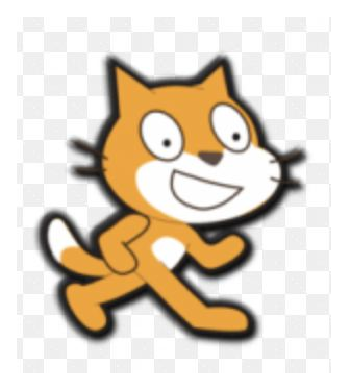
\includegraphics[width=0.8cm]{chat} indique la position de départ.

\medskip

\begin{enumerate}
\item Voir l'annexe.

%\parbox{0.5\linewidth}{On exécute le script 1 ci-contre.
%
%Représenter dans l'annexe 1  le chemin parcouru par le chat.}\hfill
%\parbox{0.48\linewidth}{
%\begin{scratch}
%\blockinit{Quand \greenflag est cliqué}
%\blockpen{stylo en position d’écriture}
%\blockmove{s’orienter à \ovaloperator{90}}
%\blockmove{avancer de \ovaloperator{80}}
%\blockrepeat{répéter \ovalnum{2} fois} 
%	{
%	\blockmove{tourner \turnleft{} de \ovalnum{90} degrés}
%	\blockmove{avancer de \ovaloperator{80}}
%	}
%\end{scratch}
%}
%\item 
%	\begin{enumerate}
%		\item Indiquer sur la copie le numéro du dessin correspondant au script 2 ci-dessous.
%	
%\parbox{0.37\linewidth}{\begin{center}Script 2 \end{center}
%
%\begin{scratch}
%\blockinit{Quand \greenflag est cliqué}
%\blockvariable{mettre \ovalvariable{pas} à \ovaloperator{\ovalvariable{80}}}
%\blockpen{stylo en position d’écriture}
%\blockmove{s’orienter à \ovaloperator{90}}
%\blockmove{avancer de \ovaloperator{pas}}
%\blockrepeat{répéter \ovalnum{2} fois} 
%	{
%	\blockmove{tourner \turnleft{} de \ovalnum{90} degrés}
%	\blockvariable{mettre \ovalvariable{pas} à \ovaloperator{\ovalvariable{pas} - \ovalnum{20}}}
%	\blockmove{avancer de \ovaloperator{pas}}
%	}
%\end{scratch}}\hfill \parbox{0.61\linewidth}{Le côté d'un carreau mesure 20 unités.
%
%\bigskip

%\begin{center}
%\psset{unit=0.4cm}
%\begin{pspicture}(20,15)
%%\psgrid
%\multido{\n=6+1}{9}{\psline[linewidth=0.5pt](\n,10)(\n,17)}
%\multido{\n=10+1}{8}{\psline[linewidth=0.5pt](6,\n)(14,\n)}
%\rput(8,11){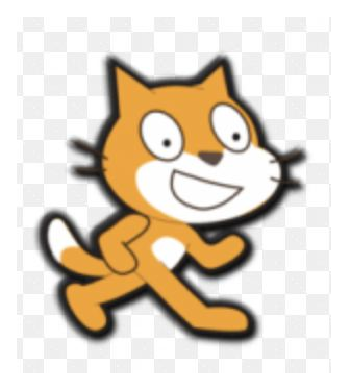
\includegraphics[width=0.3cm]{chat}}
%\rput(13,16){\large 1}
%\psline[linewidth=1.25pt](8,11)(8,15)(11,15)(11,13)
%\multido{\n=0+1}{9}{\psline[linewidth=0.5pt](\n,0)(\n,7)}
%\multido{\n=0+1}{8}{\psline[linewidth=0.5pt](0,\n)(8,\n)}
%\rput(2,1){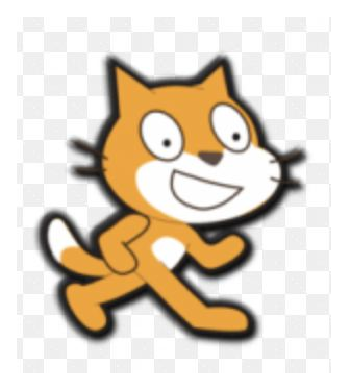
\includegraphics[width=0.3cm]{chat}}
%\rput(7,6){\large 2}
%\psline[linewidth=1.25pt](2,1)(6,1)(6,4)(4,4)
%\multido{\n=12+1}{9}{\psline[linewidth=0.5pt](\n,0)(\n,7)}
%\multido{\n=0+1}{8}{\psline[linewidth=0.5pt](12,\n)(20,\n)}
%\rput(14,1){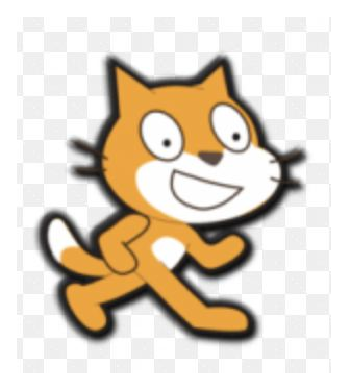
\includegraphics[width=0.3cm]{chat}}
%\rput(19,6){\large 3}
%\psline[linewidth=1.25pt](14,1)(18,1)(18,5)(14,5)
%\end{pspicture}
%\end{center}}
On avance à droite de 4 carreaux, on tourne à gauche et on avance de $80 - 20 = 60$ carreaux, on tourne à gauche et on avance de $60 - 20 = 40$ carreaux ; on a obtenu le dessin 2.
		\item Il suffit de répéter un troisième fois la boucle \og répéter \fg.
		%On souhaite modifier le script 2 pour parcourir le chemin suivant:
%\bigskip
%
%\psset{unit=0.4cm}
%\begin{center}
%\begin{pspicture}(8,7)
%\multido{\n=0+1}{9}{\psline[linewidth=0.5pt](\n,0)(\n,7)}
%\multido{\n=0+1}{8}{\psline[linewidth=0.5pt](0,\n)(8,\n)}
%\psline[linewidth=1.25pt](2,1)(6,1)(6,4)(4,4)(4,3)
%\rput(2,1){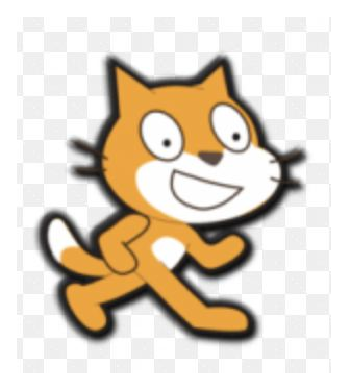
\includegraphics[width=0.4cm]{chat}}
%\end{pspicture}
%\end{center}
%
%Quelle(s) modification(s) peut-on apporter au script 2 pour parcourir ce chemin ?
\end{enumerate}
\begin{center}
\textbf{ANNEXES À RENDRE AVEC LA COPIE}

\bigskip
\textbf{Annexe 3 - question 1}

\vspace{0,5cm}

\parbox{0.45\linewidth}{Le côté d'un carreau mesure 20 unités.}\hfill
\parbox{0.52\linewidth}{\psset{unit=0.4cm}
\begin{pspicture}(8,7)
\psgrid[gridlabels=0pt,subgriddiv=1]
\psline[linecolor=blue,linewidth=1.5pt](2,1)(6,1)(6,5)(2,5)
\rput{-180}(2,5){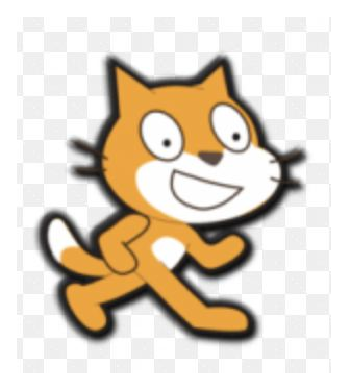
\includegraphics[width=0.4cm]{chat}}
\end{pspicture}}
\end{center}

